\documentclass[preprint,11pt,authoryear]{elsarticle}
\pdfoutput=1
\pdfminorversion=4 %had problems submitting a v1.5 pdf file with J Neurosci Methods
\usepackage{graphicx}
\usepackage{amsmath}
\usepackage{esint}
\usepackage{amssymb}
\usepackage{lineno}
\usepackage[T1]{fontenc}
\usepackage[utf8]{inputenc}
\usepackage[english]{babel}
\usepackage[]{algorithm}
\usepackage[noend]{algpseudocode}
%% natbib.sty is loaded by default. However, natbib options can be
%% provided with \biboptions{...} command. Following options are
%% valid:

%%   round  -  round parentheses are used (default)
%%   square -  square brackets are used   [option]
%%   curly  -  curly braces are used      {option}
%%   angle  -  angle brackets are used    <option>
%%   semicolon  -  multiple citations separated by semi-colon
%%   colon  - same as semicolon, an earlier confusion
%%   comma  -  separated by comma
%%   numbers-  selects numerical citations
%%   super  -  numerical citations as superscripts
%%   sort   -  sorts multiple citations according to order in ref. list
%%   sort&compress   -  like sort, but also compresses numerical citations
%%   compress - compresses without sorting
%%
%% \biboptions{comma,round}

% \biboptions{}

\bibliographystyle{elsarticle-harv}
\biboptions{square}

\renewcommand\familydefault{\sfdefault}
\usepackage[scaled]{helvet}

\usepackage{units}
\usepackage[usenames, dvipsnames]{xcolor}

\usepackage{soul}
\usepackage{placeins}

\usepackage{nameref}
\usepackage[pdftex,breaklinks=true,colorlinks=true,linkcolor=blue,citecolor=blue,urlcolor=blue,filecolor=blue,pdffitwindow,backref=true,pagebackref=false,bookmarks=true,bookmarksopen=true,bookmarksnumbered=true]{hyperref}
\usepackage[plain]{fancyref}
\usepackage{array}
\usepackage{multirow}

% Text layout
%\hoffset 2 cm
\topmargin 0.0cm
\oddsidemargin 0.5cm
\evensidemargin 0.5cm
\textwidth 16cm 
\textheight 21cm

%custom color for \hlc
\newcommand{\hlc}[2][yellow]{ {\sethlcolor{#1} \hl{#2}} }
\newcommand{\hlb}[2][blue]{ {\sethlcolor{#1} \hl{#2}} }
\newcommand{\hlr}[2][Maroon]{ {\sethlcolor{#1} \hl{#2}} }
\newcommand{\hlj}[2][OliveGreen]{ {\sethlcolor{#1} \hl{#2}} }
\newcommand{\hlR}[2][red]{ {\sethlcolor{#1} \hl{#2}} }

%boxes and highlight color for text updates, personified!
\newcommand{\ghnote}[1]{\color{white}{\hlb{GH: #1 }}\color{black}}
\newcommand{\ghtxt}[1]{{\color{blue}#1}}
\newcommand{\gtenote}[1]{\color{white}{\hlR{GTE: #1 }}\color{black}}
\newcommand{\gen}[1]{\color{white}{\hlR{GTE: #1 }}\color{black}}
\newcommand{\gtetxt}[1]{{\color{red}#1}}
\newcommand{\gex}[1]{{\color{red}#1}}
\newcommand{\genn}[1]{{\color{orange}#1}}

\newcommand{\tvnnote}[1]{\color{white}{\hlj{TVN: #1 }}\color{black}}
\newcommand{\tvntxt}[1]{{\color{OliveGreen}#1}}

%fancy ref formatting
\Frefformat{plain}{\fancyreffiglabelprefix}{Fig~#1}
\newcommand*{\Frefsecshortname}{Section}%
\Frefformat{plain}{\fancyrefseclabelprefix}{\Frefsecshortname~#1}
\Frefformat{plain}{\fancyrefeqlabelprefix}{Eq~(#1)}

%tables as in Nordlie et al. (2009)
\usepackage{tabularx}
\usepackage{colortbl}
\usepackage{morefloats}

%table formatting
\newcommand{\modelhdr}[3]{%
   \multicolumn{#1}{|l|}{%
     \color{white}\cellcolor[gray]{0.0}%
     \textbf{\makebox[0pt]{#2}\hspace{0.5\linewidth}\makebox[0pt][c]{#3}}%
   }%
}
\newcommand{\parameterhdr}[3]{%
   \multicolumn{#1}{|l|}{%
     \color{black}\cellcolor[gray]{0.8}%
     \textbf{\makebox[0pt]{#2}\hspace{0.5\linewidth}\makebox[0pt][c]{#3}}%
   }%
}
\def\tabspace{0.5ex}

\usepackage{float}
\floatstyle{plaintop}
\restylefloat{table}

\journal{nobody}


% redefinition of \author{•} because of bug (reset of \@corref missing), taken from:
% http://tex.stackexchange.com/questions/116515/elsarticle-frontmatter-corresponding-author
%
\makeatletter
\def\@author#1{\g@addto@macro\elsauthors{\normalsize%
    \def\baselinestretch{1}%
    \upshape\authorsep#1\unskip\textsuperscript{%
      \ifx\@fnmark\@empty\else\unskip\sep\@fnmark\let\sep=,\fi
      \ifx\@corref\@empty\else\unskip\sep\@corref\let\sep=,\fi
      }%
    \def\authorsep{\unskip,\space}%
    \global\let\@fnmark\@empty
    \global\let\@corref\@empty  %% Added
    \global\let\sep\@empty}%
    \@eadauthor={#1}
}
\makeatother

% - mine pakker -
\usepackage[exponent-product = \cdot]{siunitx}
\usepackage[colorinlistoftodos]{todonotes}
\usepackage[normalem]{ulem} % strikethroughs \sout{Hello World}
\usepackage{caption}
\usepackage{booktabs} % to make nice tables
\graphicspath{{Figures/}} %Setting the graphicspath
\usepackage{caption}
\usepackage{subcaption}

% - mine kommandoer - 


\begin{document}

\begin{frontmatter}

%% Title, authors and addresses

\title{Removed stuff} 

%% use the tnoteref command within \title for footnotes;
%% use the tnotetext command for the associated footnote;
%% use the fnref command within \author or \address for footnotes;
%% use the fntext command for the associated footnote;
%% use the corref command within \author for corresponding author footnotes;
%% use the cortext command for the associated footnote;
%% use the ead command for the email address,
%% and the form \ead[url] for the home page:
%%
%% \title{Title\tnoteref{label1}}
%% \tnotetext[label1]{}
%% \author{Name\corref{cor1}\fnref{label2}}
%% \ead{email address}
%% \ead[url]{home page}
%% \fntext[label2]{}
%% \cortext[cor1]{}
%% \address{Address\fnref{label3}}
%% \fntext[label3]{}

%% use optional labels to link authors explicitly to addresses:
%% \author[label1,label2]{<author name>}
%% \address[label1]{<address>}
%% \address[label2]{<address>}


%%%%%%%%%%%%%%%%%%%%%%%%%%%%%%%%%%%%%%%%%%%%%%%%%%
%%%%%%%%%%%%%%%%%%%%%%%%%%%%%%%%%%%%%%%%%%%%%%%%%%

\end{frontmatter}

%%%%%%%%%%%%%%%%%%%%%%%%%%%%%%%%%%%%%%%%%%%%%%%%%%
%%%%%%%%%%%%%%%%%%%%%%%%%%%%%%%%%%%%%%%%%%%%%%%%%%
%% Start line numbering here if you want
\linenumbers



%%%%%%%%%%%%%%%%%%%%%%%%%%%%%%%%%%%%%%%%%%%%%%%%%%
%%%%%%%%%%%%%%%%%%%%%%%%%%%%%%%%%%%%%%%%%%%%%%%%%%


%%%%%%%%%%%%%%%%%%%%%%%%%%%%%%%%%%%%%%%%%%%%%%%%%%
%%%%%%%%%%%%%%%%%%%%%%%%%%%%%%%%%%%%%%%%%%%%%%%%%%

\section{Removed}
{\bf Homogeneous:} 
On the spatial scale of a few micrometers, neural tissue is expected to be highly non-homogeneous, consisting of about 20~\% highly conductive cerebrospinal fluid (CSF) \citep{Nicholson1998, Nunez2006} with an electrical conductivity of about 1.5~S/m \citep{Martinsen2008, Logothetis2007, Miceli2017}, and about 80~\% cells, which from the viewpoint of extracellular currents are essentially non-conducting objects. 
The effective conductivity of neural tissue on the macroscale reflects this \citep{Nunez2006}: 20~\% of 1.5~S/m is 0.3~S/m, similar to what is typically measured for the neural tissue conductivity \citep{Logothetis2007, Goto2010, Miceli2017}. 
When deriving the expression for the extracellular potential, we assumed that the described microscale inhomogeneities was averaged out, and that the (effective) conductivity of neural tissue, $\sigma$, was constant. This assumption is expected to be reasonable within cortex, however, in several situations is will not be applicable.

With a spatially varying $\sigma$, we would have to derive the theory from (eq. \ref{eq:CSD} with no diffusive term):
\begin{equation}
CSD = {\bf \nabla}{\bf I} = {\bf \nabla}{\left(\sigma {\bf E}\right)} = - \nabla{\left(\sigma {\bf \nabla} \phi\right)} \\
= -\nabla \sigma \nabla \phi - \sigma \nabla^2 \phi.
\label{eq:poisson_}
\end{equation}

 A frequency dependent conductivity can be incorporated into the forward modelling scheme, essentially by solving eq.~\ref{eq:VCtheory} for each frequency component separately, that is, the transmembrane currents are transformed into the frequency domain by a Fourier Transform, and eq.~\ref{eq:VCtheory} is used with a separate conductivity for each frequency, before the signal is transformed back to the time domain \citep{Tracey2011, Miceli2017}.
Beware however that to preserve causality, that is, no signature of an event should be visible in the extracellular potential before the event has happened, one must also find the appropriate phase-shifts, for example through the Kramers–Kronig relations\citep{Martinsen2008, Miceli2017}.

\subsection*{Single-cell LFP contributions}
Excitatory synaptic inputs opens small pores (ion-channels) in the cellular membrane of the post-synaptic cell, causing positive ions to flow into the cell \citep{Kandel2012}, which, by convention, is referred to as a current sink (negative current). As we have seen, this will necessarily lead to a current source somewhere else on the cell (Sec.~\ref{sec:corrent_conservation}).  
Excitatory synaptic input to the apical dendrite of a pyramidal cell, will tend to give an apical current sink and a corresponding basal current source (Fig.~\ref{fig:dipole_basics}A), while excitatory synaptic input to the basal dendrite will give the opposite: a basal sink and an apical source (Fig.~\ref{fig:dipole_basics}B). Importantly, this means that excitatory input that simultaneously targets both the apical and the basal dendrite will give opposite source/sink patterns which will lead to substantial cancellation, and result in a much weaker contribution to the LFP (Fig.~\ref{fig:dipole_basics}C) (but see \cite{Ness2018}).
The same arguments also applies to inhibitory synaptic inputs, with the signs of the currents reversed (Fig.~\ref{fig:dipole_basics}D-F). 

Note that, for example, the LFP signature of apical excitatory synaptic input is inherently similar to that of basal inhibitory input (Fig.~\ref{fig:dipole_basics}, A versus E), and indeed, separating between cases like this poses a real challenge in interpreting LFP signals [cite]. 

Broadly speaking, neurons can be divided into two main classes: the inhibitory interneurons, and the excitatory pyramidal neurons, which make up about 20~\% and 80~\% of the total neuron numbers respectively \citep{Kandel2012}. While a typical pyramidal neuron has a clear axis of orientation, that is, the apical dendrites of close-by pyramidal neurons tend to be oriented in the same direction, this is much less true for interneurons, which often lack any clear orientational specificity. This has important consequences for their ability to contribute to the LFP: 


\begin{figure}[ht!]
\begin{center}
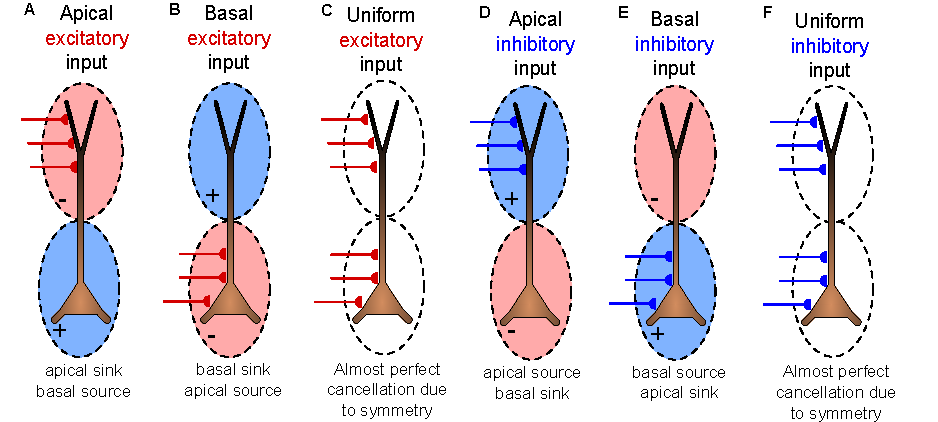
\includegraphics[width=0.8\textwidth]{dipole_basics}
\end{center}
\caption{\textbf{Basic building blocks of the LFP.} Illustration of the LFP at a snapshot in time in a region around a pyramidal cell in response to different types of synaptic input.  
The LFP signature depends on the type of synaptic input (excitatory or inhibitory), and the location (apical, basal, uniform), but also, to a lesser degree, to many other parameters of the cells and synapses.
}
\label{fig:dipole_basics}
\end{figure}

\section{The vital role of current conservation}
\label{sec:corrent_conservation}
Neural simulations with detailed multi-compartment cell models is based on solving the cable equation (Chapter in this book?), with a built-in assumption of current conservation \citep{Koch1999}. Current conservation implies that the summed current across the cellular membrane will, at any given time, sum to zero,
\begin{equation}
 \sum_k I_k = 0.
 \label{eq:current_conservation}
\end{equation}
Note that the capacitive currents have a vital role in ensuring this current conservation: the membrane potential is caused by a slight charge imbalance between the inside and the outside of the cell, and all this surplus charge is expected to be distributed on the cellular membrane, where all the surplus charge on the inside of the cellular membrane (negative during the resting state) is exactly balanced by an equal amount of charge of the opposite polarity on the outside of the cellular membrane (Fig.~\ref{fig:capacitive_currents}A) [cite]. 
As current pass through the membrane, or from one part of the cell to another, the amount of surplus charge on the inside of the cellular membrane changes (Fig.~\ref{fig:capacitive_currents}B), which immediately results in a corresponding change in the amount of charge on the outside of the cellular membrane (Fig.~\ref{fig:capacitive_currents}C). Such changes in the amount of surplus charge distributed along the outside of the cellular membrane are what is called capacitive currents, and they ensure that eq.~\ref{eq:current_conservation} is always fulfilled.
Current conservation has far-reaching consequences for extracellular potentials, that we will illustrate with three examples.
\begin{figure}[ht!]
\begin{center}
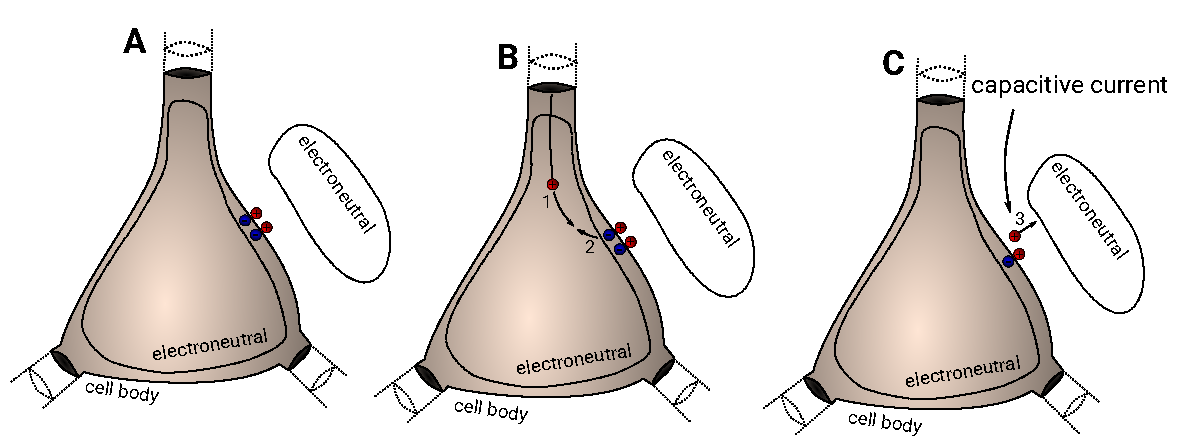
\includegraphics[width=1\textwidth]{capacitive_currents}
\end{center}
\caption{\textbf{Capacitive currents ensures current conservation.
\tvnnote{Mention time scale of this?}
\tvnnote{Not sure if this makes sense to include?}
}}
\label{fig:capacitive_currents}
\end{figure}

\subsection*{Illustration with point-neuron model}
Consider for example the often-used point-neuron models \citep{Sterratt2011}. Since they have only one compartment, eq.~\ref{eq:current_conservation} demands that there should be no net transmembrane current, implying no extracellular potentials (see eq.~\ref{eq:VCtheory}). This means that, while point-neurons have an important role to play in investigating neural network dynamics \citep{Einevoll2019}, they are in general incapable of producing extracellular potentials (Fig.~\ref{fig:EP_morph}A; see however \cite{Mazzoni2015, Hagen2016}). 

\begin{figure}[ht!]
\begin{center}
\includegraphics[width=0.6\textwidth]{dipoles}
\end{center}
\caption{\textbf{Effect of current conservation on extracellular potentials.} 
Illustration of synaptic input to three different types of cell models (top row), with the resulting extracellular potentials (bottom row). 
A: Point neurons have no net currents, and therefore cause no extracellular potentials. B: Two-compartment neuron models have two opposite currents
of identical magnitude, and cause dipolar extracellular potentials. C: Multi-compartment neuron models \citep{Hay2011} give rise to extracellular potentials with complex (but mostly dipolar-like) shapes.}
\label{fig:EP_morph_}
\end{figure}


\subsection*{Illustration with two-compartment model}
Consider now a cell model with two cellular compartments. Current conservation, through eq.~\ref{eq:current_conservation}, then implies $I_1 + I_2 = 0$, which in combination with eq.~\ref{eq:VCtheory} gives,
\begin{equation}
 \phi ({\bf r}) = \frac{I_1}{4\pi {\bf |r-r_1|} \sigma} + \frac{-I_1}{4\pi {\bf |r-r_2|} \sigma} = \frac{I_1}{4\pi \sigma}\left ( \frac{1}{{\bf |r-r_1|}} - \frac{1}{{\bf |r-r_2|}}\right ).
\end{equation}
In words, the exact same amount of current that goes into one compartment, goes out of the other, resulting in a current dipole (Fig.~\ref{fig:EP_morph}B).

\subsection*{Illustration with multi-compartment cell model}
For multi-compartment cell models, the situation becomes more complex, but current conservation is still key in shaping extracellular potentials, and ensures that there are no current monopoles. This means that in general neural activity can be expected to cause both negative and positive currents, resulting in both positive and negative extracellular potentials (Fig.~\ref{fig:EP_morph}C).

LFP is low-pass filtered, but note that spikes, like delta-funcitons, have substantial power in low-frequencies.

\subsection*{Correlations boost LFP signals}
Correlations have been demonstrated to play a vital role, and can increase the amplitude of the LFP by orders of magnitude \citep{Linden2011, Leski2013}. The effect is in principle easy to understand (Fig.~\ref{fig:correlation_effect}).

\tvnnote{Could have (i) no figure, (ii) remake figure from Linden et al., (iii) make simple illustration figure of underlying reason for boost?} 

\begin{figure}[ht!]
\begin{center}
\includegraphics[width=0.5\textwidth]{correlation_jitter}
\end{center}
\caption{\textbf{[Placeholder] Effect of correlation}. Simple illustration of correlation effect. A single instance of a toy ''synaptic input`` (A), is used as a building block for creating ''spike trains`` which are summed into compound signals (B). The ''spike trains`` are either completely uncorrelated, that is, 20 random ''spike trains`` are summed (blue), or completely correlated, that is a single ''spike train`` is summed 20 times (red). Although the blue and red lines had exactly the same number of ''spikes`` (the integral over the signals are identical), the power-spectral density (PSD) of the correlated case is an order of magnitude larger than the uncorrelated case (panel D; red versus blue).}
\label{fig:correlation_effect}
\end{figure}



\subsection{Intrinsic dendritic filtering}
As a thought experiment, imagine a synapse that supplies a cell with a sinusoidal synaptic current. From current conservation we know that this input current must be exactly matched by the ensuing return currents, but how much of the current will leave the membrane in the immediate vicinity of the synapse, and how much will spread through the cell and leave through more distant parts of the membrane? 
%If, for example, the synapse is located on a thin dendritic branch it perhaps seems intuitive that much of the current would move axially within the cell and leave the membrane through the somatic region, where there is much more available membrane area for the current to leave through.
There are basically three ways that currents can leave a cellular compartment. First, there are two types of membrane currents, namely ionic and capacitive.
Ionic currents tend to be on the form $I_i(t)=g \cdot (V(t) - E_{rev})$ for so-called passive currents, while for active currents, $g$ would be time dependent.
The capacitive current at position ${\bf r}$ along the membrane at time $t$, is given by \cite{Koch1999},
\begin{equation}
I_c ({\bf r}, t) = c_m\, \tfrac{dV({\bf r}, t)}{dt},
\end{equation}
with membrane capacitance $c_m$. Lastly, there are axial currents, essentially given by Ohm's law, $I_a = \Delta V / r_a$, where $\Delta V$ is the difference in potential between two neigbouring compartments, and $r_a$ is the resistance between them.

Note that, in contrast to ionic and axial currents, capacitive currents are proportional to the time derivative of the membrane potential, implying that if the hypothetical sinusoidal synapse had a high frequency (say 100-1000~Hz), the
membrane would in effect be ''leakier`` than it would be for a low frequency current (say 1-10~Hz), while the axial resistance would be the same in the two cases. Effectively, this shifts the return currents closer to the input site for higher frequencies than for lower frequencies. 

Passive cell models, that is, cell models without voltage-dependent ion channels (see Sec.~\ref{sec:active}) are linear, meaning that each frequency component can be solved separately, and since all signals can be represented as a sum of sinusoids, this means that as a signal propagates through a cell, it will become increasingly low-pass filtered. This effect is called intrinsic dendritic filtering \citep{Linden2010}, and it can have a substantial influence on extracellular potentials (Fig.~\ref{fig:intrinsic},~\ref{fig:intrinsic2}).
\begin{figure}[ht!]
\begin{center}
\includegraphics[width=0.5\textwidth]{intrinsic_dendritic_filtering.png}
\end{center}
\caption{\textbf{Intrinsic dendritic filtering} From \cite{Linden2010}.}
\label{fig:intrinsic}
\end{figure}

\begin{figure}[ht!]
\begin{center}
\includegraphics[width=0.8\textwidth]{hay_intrinsic.png}
\end{center}
\caption{\textbf{Intrinsic dendritic filtering} From \cite{Ness2016}.}
\label{fig:intrinsic2}
\end{figure}

\subsection{Old derivation of VC-theory}
\begin{equation}
\nabla^2 \phi = - CSD/\sigma,
\label{eq:trygve}
\end{equation}
where we have introduced the electrical field 

${\bf E}={\bf \nabla} \phi$ \tvnnote{Comment on this? Maxwell -> quasistatic -> cross-product = 0 implies E is gradient of scalar function. Is anything gained by introducing  {\bf E} at all, when we already have $\phi$? Or how about using {\bf E} instead of $\nabla\phi$ from the start?}, and for now assumed that the conductivity, $\sigma$, is a scalar constant. We integrate each side of this equation over a 3D volume,
\begin{equation}
\iiint_V E({\bf r}) \,d^3V =  - \frac{1}{\sigma} \iiint_V \ CSD({\bf r}) \, d^3V.
\label{eq:trygve2}
\end{equation}
If we consider the simplest possible case of a single point current source $I_1$ in ${\bf r}=0$, the right hand side becomes $-I_1/\sigma$. By Gauss' theorem, we can convert the left hand side to a surface integral, and get:
\begin{equation}
\iiint_V E(r) \,d^3V =  \oiint_{S} E(r) \,d^2S = 4\pi r^2 E(r) = 4\pi r^2 \frac{d\phi}{dr} = -\frac{I_1}{\sigma},
\label{eq:trygve3}
\end{equation}
where we have exploited the spherical symmetry of the problem. Finally, integration with respect to $r$ gives us

\subsection{Anisotropy equations}
\begin{equation}
\phi(x,y,z) = \frac{i_e}{4\pi(\sigma_y\sigma_z x^2 + \sigma_x\sigma_z y^2 + \sigma_x\sigma_y z^2)}.
\end{equation}
In cortex, it has been found that the conductivity is in fact about 50 \% higher along the depth axis, that is, parallel to the axis of the pyramidal dendrites \citep{Goto2010}, however, the overall effect of this on extracellular potentials appears quite weak \citep{Ness2015}.

\section{Electrodes}
\tvnnote{Do we want this part?}
\ghnote{I don't. Besides, we probably do not have space to include it.}
\subsection{Size}
Spatial averaging matters, but is relatively easily studied
\subsection{Frequency filtering}
Nelson says no (for recording electrodes) \citep{Nelson2010}

\subsection*{Effect of spikes and active conductances}
\label{sec:active}
\ghnote{Perhaps make this stuff more compact, and not have it as separate subsection?} \tvnnote{I kind off made it more compact, but also expanded the text a bit.}
%Active conductances can affect LFP signals in different ways, for example through the presence of somatic action potentials, dendritic calcium spikes or subthreshold processing of synaptic inputs.
Somatic action potentials are typically not expected to have an important role in shaping cortical LFP signals for several reasons \citep{Einevoll2013, Haider2016}, for example, their very short duration with both positive and negative phases (Fig.~\ref{fig:EP_morph}E) would require extreme synchrony to sum constructively in the LFP, and their high frequency content is to a large degree removed from LFPs during low-pass filtering. 
There are, however, indications that in particular the relatively long-lasting after-hyperpolarization might, at least in some cases, have a role in shaping the LFP, see for example \cite{Reimann2013}.
Note that in the hippocampus the highly synchronized spikes found during sharp wave ripples are expected to strongly shape the LFP \citep{Schomburg2012, Luo2018}. 

It has been demonstrated by \cite{Suzuki2017} that calcium spikes can make sizable contributions to the LFP and ECoG signals, which opens up for exciting research opportunities, given the assumed important physiological role of such calcium spikes\tvnnote{remove?}.

Subthreshold active conductances can also be expected to affect the LFP, and in particular the hyperpolarization-activated cation channel I$_{\rm h}$ might play a key role in this, see \cite{Ness2016, Ness2018}.
\begin{figure}[!ht]
\begin{center}
\includegraphics[width=1\textwidth]{population_EEG_MEG.png}
%\includegraphics[width=1\textwidth]{PC_versus_IN}
\end{center}
\caption{\textbf{Extracellular potentials from different waves of synaptic input}. Different brain signals from separate waves of synaptic input to 10 000 layer 5 pyramidal cells from rat \citep{Hay2011}.
{\bf A}: A subset of 100 pyramidal cells, with the LFP electrode locations indicated in the center (colored dots).
{\bf B}: Depth-resolved synaptic inputs arrive in three waves, first targeting the basal dendrites (t=$\sim$60~ms), then the apical dendrites (t=$\sim$130~ms), and lastly uniformly across the entire depth (t=$\sim$200~ms). Note that all synaptic input is pre-defined, that is, there is no network activity.
{\bf C}: The LFP at different depths (colors correspond to dots in panel A)
{\bf D}: The four-sphere head model with two orientations of the neural population, either radial, mimicing a population in a gyrus (top) or tangential, mimicing a population in a sulcus (bottom).
{\bf E}: A snapshot of the EEG signal at the head surface for apical input (time marked with dotted line in panel B and C), for a radial population (top) or tangential population (bottom).
}
\label{fig:LFP_EEG}
\end{figure}



\subsection*{Voltage-sensitive dye imaging}
In principle easy to model, just area-weighted membrane potential
\subsection*{Calcium imaging}
Depends on cell models with good calcium dynamics, which is a weakness of many present models.
\subsection*{fMRI}
Underlying mechanism for other signals seems clear, but this is not so for fMRI. fMRI is thought to be a measure of ''metabolic cost``, but appears cell-type dependent, with an important role of NPY interneurons.




\section*{References}
\label{sec:bibliography}
\bibliography{ECS_bookchapter.bib}

\end{document}  
